\chapter{Literature Review}

\section{Literature Introduction}

This section of this paper will be focusing on the literature and the relevant research related to web development and procurement of easy to use web form systems. This includes the information that was able to be recovered from scholarly articles and books on the history, current implementations, as well as theoretical system designs of websites for the near future; but also includes some of the conflicting design philosophies behind stack development and why certain tools are developed for different tasks depending on an application's needs or demands.

\section{Theory of System Design}

As demand for services on the internet have grown, the complexity and scale of web applications have grown with this demand \cite{Ivory_Megraw_2005}. Early websites used an incredibly simplistic and static design of the 90s, where today’s responsive and fluid feel designs are now commonplace \cite{Chen_Tang_Wang_Zhao_Guo_2016}. With the advent of mass scale online sale and large user bases, internal systems within sites have also grown significantly to accommodate traffic that was not possible in the 90s; with that growth has come a variety of toolsets and frameworks for developers to pull on and utilise \cite{Chen_Tang_Wang_Zhao_Guo_2016, Abdullah_Zeki_2014, Ivory_Megraw_2005}. These early designs of the 90s were both incredibly difficult for users to have high interaction with as well as generally were hard on eyes due to the difficulty of reading large blocks of text with bright backgrounds \cite{Chen_Tang_Wang_Zhao_Guo_2016}. These sites also did not provide any sort of backend systems but were generally static pages designed simply to serve a piece of written information to the user and not much else \cite{Ivory_Megraw_2005}.
\newline
\newline
An incredibly famous example of facing scalability issues with the growth of the internet is Facebook.com \cite{Abdullah_Zeki_2014, Stolberg_2009}. Facebook is a prime example of a social media company that needed to develop many of the toolsets that are now used to solve many scalability issues including both frontend frameworks such as React and back-end toolsets like GraphQL as discussed in section 2.3 and 2.5 \cite{Abdullah_Zeki_2014, Brito_Valente_2020, Xu_2021}. This was to meet a sizable user base that had never quite been seen before \cite{Chen1_Ji1_Fan1_Zhan2_2017}. All this user growth required a new way of approaching problems to make Facebook.com never go down and always have a modern look and feel to it, while using frameworks such as React to create easily readable code as well as an easy to maintain codebase \cite{Chen1_Ji1_Fan1_Zhan2_2017}. This includes the moving away from large scale applications that require stronger and more powerful computers to handle all incoming and outgoing requests to a micro-service system; thus making it so that if one service goes down the whole website does not crash or lead to catastrophic failure \cite{Villamizar_Garcés_Castro_Salamanca_Casallas_2017}.
\newline
\newline
Monolithic project structures do have the positive of being far easier to understand on small scales allowing for rapid development of many feature sets in short amounts of time \cite{Combe_Martin_Di_Pietro_2016, Villamizar_Garcés_Castro_Salamanca_Casallas_2017}. This makes it so that a new team of developers do not have to focus on developing gateway services or large scale data routing until later in the project's scope \cite{Villamizar_Garcés_Castro_Salamanca_Casallas_2017}. This also means that, when using cloud computing to deploy an app, it will not require many computers but rather a stronger one, which can have the benefit of being cheaper if the number of clients accessing the system is always small \cite{Villamizar_Garcés_Castro_Salamanca_Casallas_2017}.
\newline
\newline
With the growth of cloud computing however, micro-service architecture is the way of the future and allows for dockerization of code \cite{Combe_Martin_Di_Pietro_2016}. This allows for deployment of nearly infinite amounts of micro computers able to handle more and more requests, scaling with the user base of a website \cite{Combe_Martin_Di_Pietro_2016}. This also allows for each machine to be identical to the last while not needing access to the whole lower level operating system that a virtual machine provides \cite{Combe_Martin_Di_Pietro_2016}. A web application in practice should never need raw instructions to be executed on a GPU or CPU, but rather simply need a level of higher abstraction to render a web page for a user and provide back a set of JSON values \cite{Combe_Martin_Di_Pietro_2016}. Identical machines created using docker and similar containers makes all machines equal in creation to deletion, thus ensuring every instruction is always executed the same \cite{Combe_Martin_Di_Pietro_2016}.
\newline
\newline
Developing along this level of containerisation also allows for easier continuous integration (CI/CD) development \cite{Stolberg_2009, Red_Hat_Devops_2022}. Each service as its version controlled can be run against a series of tests and network tests to see how it interacts with all other services before deployment to the production environment \cite{Red_Hat_Devops_2022}. Without this level of automated testing, developers would not be able to assess how a new set of code will work on the internet \cite{Stolberg_2009}. This also provides security as new features are rolled out to the public and protects business interests \cite{Combe_Martin_Di_Pietro_2016}.

\section{REST and GraphQL}

Almost all websites today now need to have custom sets of data specific to user data and actions that can only be performed by specific users. To solve the issue of querying for data from a database with using only user-specific permissions, REST and the more modern solution of GraphQL were created \cite{Brito_Valente_2020}. Representational State Transfer (REST) takes the approach of giving a user a specific set of information, often in the form of JSON, when provided a very specific set of instructions to an endpoint exposed to the web \cite{Brito_Valente_2020}. This plays extremely well with multi-system architectures as shown earlier as multiple computers can be running on each endpoint without collisions to each request made \cite{Villamizar_Garcés_Castro_Salamanca_Casallas_2017}. This is from REST’s original  design of being “intended to improve performance, availability, and scalability” \cite{Brito_Valente_2020}. This also gives the added advantage of having an easy to implement design from dozens of libraries and implementations for every mainstream language \cite{Chen1_Ji1_Fan1_Zhan2_2017}. Back-end endpoints can be configured and removed as an application grows as well, thus giving programmers fine-grained control over their stack \cite{Chen1_Ji1_Fan1_Zhan2_2017}.

\begin{figure}[H]
\centering
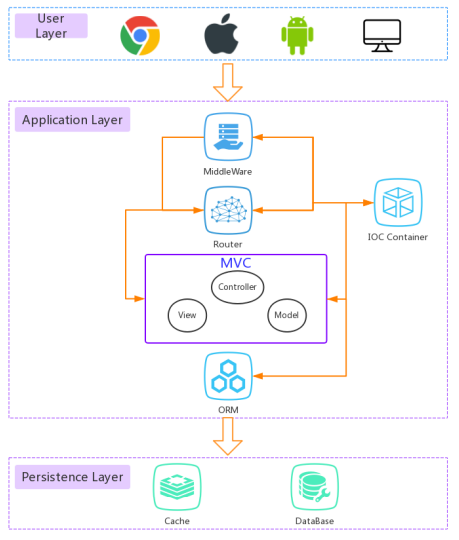
\includegraphics[width=13.5cm]{myReport/images/mvcREST.png}
\caption{Application diagram of a modern web service application stack \cite{Chen1_Ji1_Fan1_Zhan2_2017}}
\label{fig:mvcREST}
\end{figure}

As shown in Figure \ref{fig:mvcREST}, the middleware allows for the protection of the database and caches while providing information to the client \cite{Chen1_Ji1_Fan1_Zhan2_2017}. It is irrelevant how the front end application looks if the back-end always provides information correctly from the database and can use a model-view controller to maintain security over the database \cite{Chen1_Ji1_Fan1_Zhan2_2017}.
\newline
\newline
REST allows for 4 types of interactions with a back-end API to change data within a database. These CRUD functions would be to CREATE, READ, UPDATE, and DELETE \cite{Hartig_Pérez_2018}. This makes it so that a user or front end website can provide to a given endpoint all the necessary information such as a user id or query data set that needs to be altered in the database and then that function is done via the back-end \cite{Haupt_Leymann_Scherer_Vukojevic-Haupt_2017}. This is near infinitely scalable so long as a database can handle a given number of transactions being made at a given time so long as the time it takes for inter-service calls to not be too great in scale \cite{Li_Manoharan_2013}. The greatest slowdowns with the paradigm of design is when a service has to wait on potentially many services down and there is large lookup times within each one waiting for a response from another service \cite{Li_Manoharan_2013}.
\newline
\newline
Developers will often choose to document their back-end endpoints and a more common practice now developing is to use an auto documentation tool such as swagger \cite{Haupt_Leymann_Scherer_Vukojevic-Haupt_2017}. Swagger provides an easy to visualise page of all endpoints exposed and their given function or relational action to the database \cite{Haupt_Leymann_Scherer_Vukojevic-Haupt_2017}. This is incredibly important especially in large scale applications with potentially hundreds of micro-services and dozens of endpoints per service \cite{Haupt_Leymann_Scherer_Vukojevic-Haupt_2017, Li_Manoharan_2013}. The alternative is the have custom create documentation tools that are for incredible scale projects or to utilize a single endpoint to avoid all this and use a query system instead \cite{Haupt_Leymann_Scherer_Vukojevic-Haupt_2017, Stubailo_2021}. Not having to track many endpoints and instead query all data from 1 place is what GraphQL was created to solve \cite{Brito_Valente_2020, Stubailo_2021}.
\newline
\newline
GraphQL is a more modern way of querying for information on the back-end and takes the approach of giving more data than necessary in a given request \cite{Brito_Valente_2020, Stubailo_2021}. Designed at Facebook originally to meet larger and larger scale demands from a growing user base, GraphQL has since been open source and is available to the public for many modern web frameworks \cite{Abdullah_Zeki_2014}. In design, GraphQL instead makes a single endpoint for all requests to collect data from \cite{Brito_Mombach_Valente_2019, Brito_Valente_2020}.  Querying for data is then done through a pre-generated graph provided by the back-end code \cite{Brito_Mombach_Valente_2019}.  This makes it incredibly easy for development time as well as the time it takes for new developers to learn and migrate from old REST based systems \cite{Hartig_Pérez_2018}.  The query language of GraphQL is also heavily SQL inspired making it easy for implementation of requests and gives a sense of familiarity when working with endpoints of this fashion \cite{Brito_Mombach_Valente_2019}.

\begin{figure}[H]
\centering
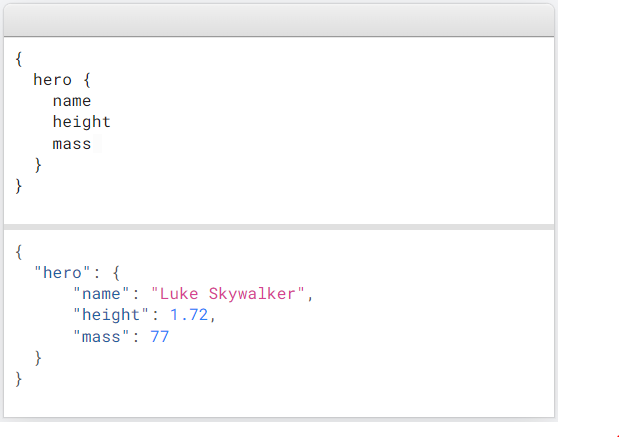
\includegraphics[width=15cm]{myReport/images/GraphQL_Example.png}
\caption{Sample query using GraphQL \cite{GraphQL}}
\label{fig:graphQL_example}
\end{figure}

As can be seen in Figure \ref{fig:graphQL_example}, any information a client needs can be queried using a simple syntax to ask for all fields necessary. This makes it such that only information needed for a particular task is provided rather than the approach of REST throwing more information than necessary at a client \cite{Brito_Mombach_Valente_2019}. In Figure \ref{fig:graphQL_example}, the top box queries for all fields the client is requesting and the bottom box serves back the results of those fields from the database \cite{GraphQL}.
\newline
\newline
In a comparison of REST and GraphQL, it can be seen that they each provide benefits and pitfalls to web application stacks \cite{Stubailo_2021}.  GraphQL’s biggest strength is that since it does not need to provide a linear list of endpoints, thus routing is incredibly easy from a back-end developer’s perspective \cite{Stubailo_2021}. This also makes responses predictable as everything is retrieved using a GraphQL schema \cite{Brito_Mombach_Valente_2019, Stubailo_2021}. Comparing this to a REST approach, it is far easier for a developer to envision the early stages of their project and can manipulate different endpoints as necessary as a project grows in scale and complexity \cite{Stubailo_2021}. All endpoints can be developed independently by separate teams focused on different tasks with little worry about destroying the entire application at any given moment \cite{Brito_Mombach_Valente_2019, GraphQL, Stubailo_2021}.

\section{Django and Flask}

In order to serve data from a database in a secure and reliable way, there have been a variety of libraries developed to aid developers in accomplishing this task \cite{Chen1_Ji1_Fan1_Zhan2_2017}. Some of the most popular frameworks are Rails, Node.js, Django, Flask, Spring Boot, .NET, and Laravel \cite{Challapalli_Kaushik_Suman_Shivahare_Bibhu_Gupta_2021, Ravindran_2018, Clark}. Given the ease of development time and simplicity provided by the Python programming language, there have been a few incredibly popular web frameworks to have arisen over the years \cite{Ravindran_2018}. Given the widespread usage of the two most used frameworks however, there will be emphasis on Django and Flask as not only are these frameworks some of the most popular frameworks, but also have the most research provided about each one respectively \cite{Chou_Chen_Ding_Tu_Xu_2013}.
\newline
\newline
Django is designed to be a "batteries-included" library with little to no effort needed for setup \cite{Ravindran_2018, Challapalli_Kaushik_Suman_Shivahare_Bibhu_Gupta_2021}. Django is built using a common practice MVC system with a model, view, and controller based design \cite{Chou_Chen_Ding_Tu_Xu_2013}. Models can be created to represent objects within a database and then the Django framework will automatically store and manipulate those tables as needed via a view \cite{Ravindran_2018}. To then call a view, an endpoint can then be exposed and have the function linked to it within the simple app created \cite{Ravindran_2018}. This is what Django developers call as "batteries-included", as the framework does most of the heavy lifting for a developer and all that is needed is instructions for what the programmer wants from their web application \cite{Ravindran_2018, Challapalli_Kaushik_Suman_Shivahare_Bibhu_Gupta_2021}.
\newline
\newline
One of the biggest driving supporting design choices for many developers is the reasoning for using Django for its ORM (Object Relational Mapping) system \cite{Khatri_Johns_2023}. This layer provides a complete mapping of classes in Python code to be converted to database structures in a complete abstraction without the programmer ever needing to worry about any of the details between \cite{Chou_Chen_Ding_Tu_Xu_2013}. Along with that batteries-included design of providing an ORM, this also gives the web developer near unparalleled security \cite{Chou_Chen_Ding_Tu_Xu_2013}. This ORM will also provide security against SQL injection attacks, as discussed later in section 2.6 \cite{Li_Manoharan_2013, Chen_Tang_Wang_Zhao_Guo_2016}. Due to the open source nature of Django, it makes it so that security flaws are easily reported and patched in a short period of time compared to private corporate solutions \cite{Chou_Chen_Ding_Tu_Xu_2013}. Some of the security options include ensuring that static files are delivered to clients in a non debug mode, making it so that Nginx and other system API routers are able to not expose back-end information to a web fetch request \cite{Khatri_Johns_2023}.
\newline
\newline
Flask is a slightly older web framework originally developed in 2004 \cite{Ravindran_2018}. Flask is popular for its long time development and support but also the simplicity afforded to the programmer. Flask is a very lightweight API that does not provide any database libraries or form abstraction layers that are fundamental to Django \cite{Dugar_2018, Ravindran_2018}. This is much better for web applications that need a much finer level control of the back-end data manipulation as well as how JSON responses are sent back to request parties \cite{Dugar_2018}.
\newline
\newline
Flask gained a lot of traction with the introduction of the Jinja templating library similar to the design of Django’s templating system \cite{Dugar_2018, Ravindran_2018}. One of the bigger advantages to using Jinja over Django is that it is optional for serving templated responses, as some web applications, particularly examples like book databases, do not need a consistent return state for every single request \cite{Dugar_2018}. With Jinja2, the library also introduced the ability for most of a developer's pythonic code to be run in a templated system if needed allowing for greater extensibility \cite{Dugar_2018}. The downside to this approach over Django’s system is that this makes it harder for logic to be split and understood from a maintenance standpoint \cite{Dugar_2018}.
\newline
\newline
In comparison of the two, both libraries offer features and systems that can be desirable to a developer depending on what is being created \cite{Khatri_Johns_2023}. Django’s security is far better out of the box and requires little configuration at all compared to Flask \cite{Khatri_Johns_2023}. Django’s biggest driver for projects however, is that it supports multi-page applications \cite{Ravindran_2018}. Flask does not have the ability to create large and complex applications easily and is more more driven towards small micro-services that require far more tailoring \cite{Chou_Chen_Ding_Tu_Xu_2013, Khatri_Johns_2023}. Coupled with the fact that Flask really only has support for NoSQL databases at best, it makes it also hard to handle large amounts of data and certainly lacks the ability to add extra support for database caching such as Redis \cite{Khatri_Johns_2023}.
\newline
\newline
On the other hand, Flask does create the perfect handling for small applications that do not need to serve large volumes of information \cite{Khatri_Johns_2023}. This is great for internal projects in companies as well as small hobby projects that really shouldn't need a large library to power such applications \cite{Challapalli_Kaushik_Suman_Shivahare_Bibhu_Gupta_2021, Ravindran_2018, Khatri_Johns_2023}.

\section{Front-end Framework Choice}

Developing front-end rendering systems has led to a variety of many options to choose from compared to the early days of simple HTML and CSS \cite{Xu_2021}.  Now there are a variety of JavaScript based options available to developers along with the newer language of Typescript which is a super set of JavaScript \cite{Constantinides_2004}. There are a variety of libraries that have been developed to solve the needs of developers as well as automate tasks such as hydrating the DOM (Document Object Model) \cite{Xu_2021}.
\newline
\newline
One of the most popular frameworks is React, a library developed by Facebook for web applications and eventual support for native mobile apps as well \cite{Xu_2021, Clark}. React has grown immensely in popularity due to reliable support as well as the incredibly massive ecosystem by many developers \cite{Clark}. React was first released to the public in 2013 as an open-source library \cite{Clark, Dhaduk_2023}. One of the most notable features that was pioneered early was React’s component design system using functional components to construct UI elements and useRef to store information within functional elements \cite{Clark}.

\pagebreak
\begin{figure}[H]
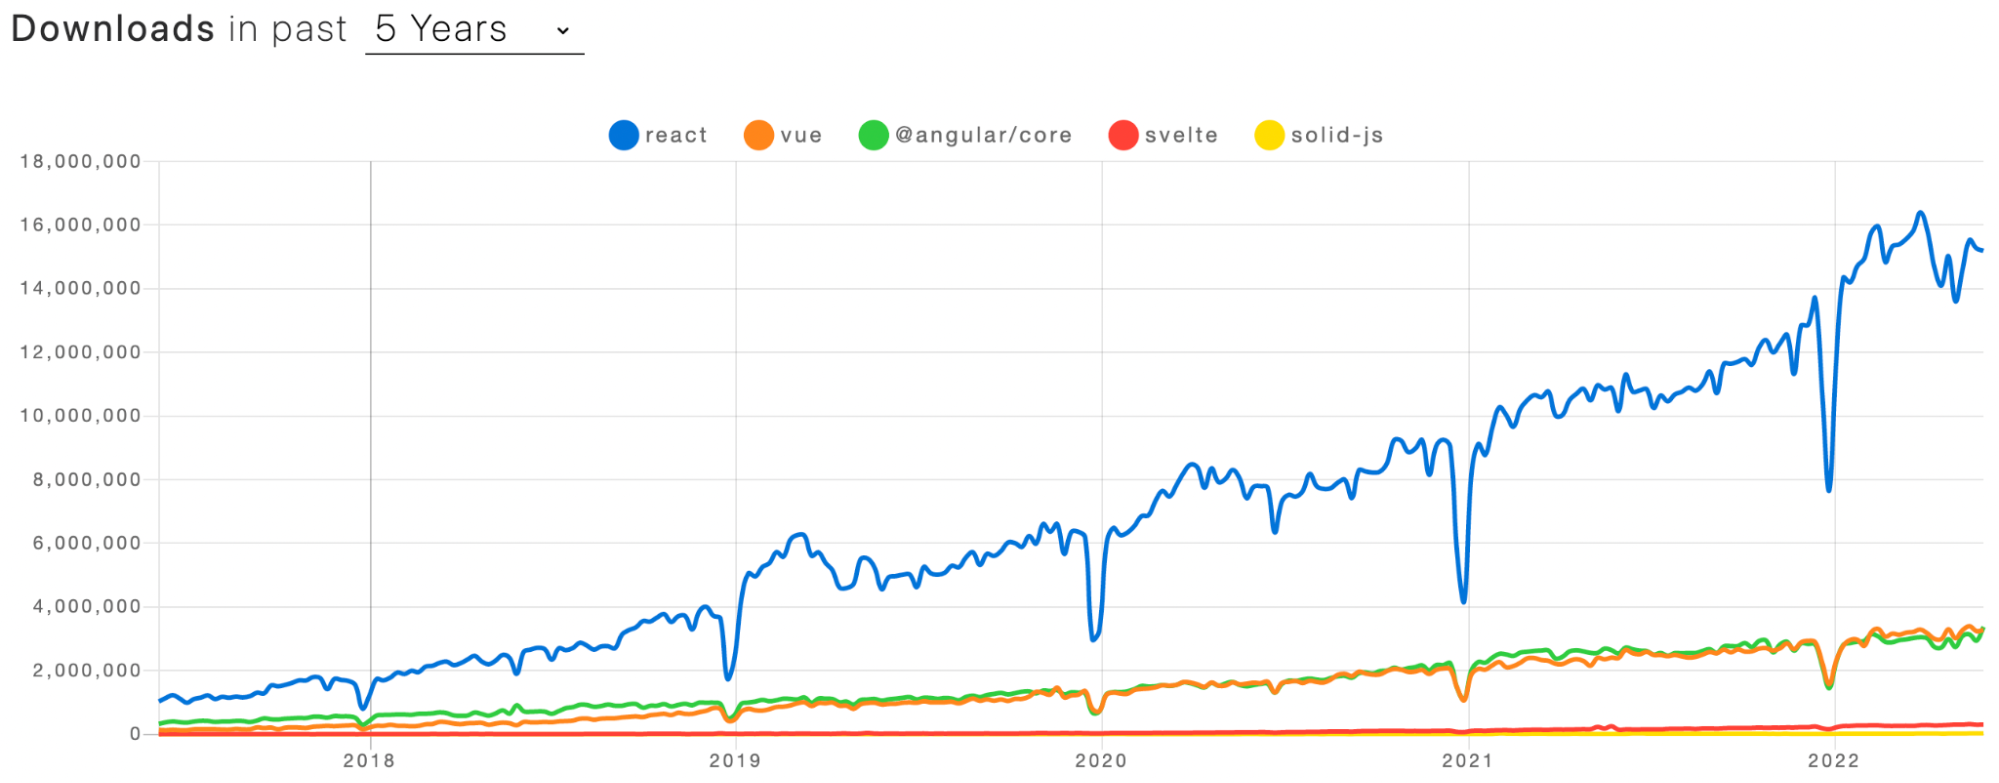
\includegraphics[width=15cm]{myReport/images/image2.png}
\caption{Popularity of frontend framework based on NPM downloads \cite{Krotoff}}
\label{fig:npmPop}
\end{figure}

As can be seen from Figure \ref{fig:npmPop}, react has maintained its popularity over the years based on downloads and supported NPM packages \cite{Krotoff}. This is partially due to how React is one of the oldest frameworks, thus creating more libraries and community support than many other modern tools \cite{Krotoff}. With Angular and Vue being the second most popular frameworks, angular in particular comes with a significant amount of more robust and powerful features for developers \cite{Xu_2021}.
\newline
\newline
With the release of Angular in 2016, it was one of the first large scale JavaScript frameworks to provide programmers far more tools than just UI tooling \cite{Dhaduk_2023}. Angular provides developers the ability to use dependency injection and rapid server side rendering for making back-ends and front-ends blend more seamlessly \cite{Dhaduk_2023, Xu_2021}. This creates the benefit of developers having a much greater toolset at their disposal and less need to worry about errors with data in transit between services \cite{Dhaduk_2023}. Providing such strict object manipulation also allows for easy AJAX development for programmers on front-end applications, thus removing the need to worry about virtual DOM issues if a page is large and has to wait for many asynchronous functions to finish before hydrating \cite{Dhaduk_2023, Xu_2021}.

\section{Database Design Options}

One of the most difficult options is trying to determine what kind of database suite would work best for an application’s needs \cite{Li_Manoharan_2013}.  While SQL has been around since the 70s, there have been various advancements made in attempts to do large data storage such as document-driven designs \cite{Chen_Tang_Wang_Zhao_Guo_2016, Li_Manoharan_2013}. There is also the more recent development of caching type databases that store the most accessed data within memory of the computer rather than disk, leading to significant data accelerations for certain workloads \cite{Li_Manoharan_2013}. The most popular of these choices for memory driven databases is Redis \cite{Chen_Tang_Wang_Zhao_Guo_2016}.

\begin{table}[ht]
\centering
\begin{tabular}{c|cccccc}
\multirow{2}{*}{Database} & \multicolumn{6}{c}{Number of Keys to Fetch} \\
& 10 & 50 & 100 & 1000 & 10000 & 100000 \\
\hline
MongoDB & 4 & 4 & 5 & 19 & 98 & 702 \\
RavenDB & 101 & 113 & 115 & 116 & 136 & 591 \\
CouchDB & 67 & 196 & 19 & 173 & 1063 & 9512 \\
Cassandra & 47 & 50 & 55 & 76 & 237 & 709 \\
Hypertable & 3 & 3 & 3 & 5 & 25 & 159 \\
MS SQL Express & 4 & 4 & 4 & 4 & 11 & 76 \\
\end{tabular}
\caption{Time for all key fetch times (MS) \cite{Li_Manoharan_2013}}
\label{tab:fetch_times_db}
\end{table}

As can be seen in Table \ref{tab:fetch_times_db}, fetch times for whole tables is many thousands of times faster using SQL than it is using a NoSQL database \cite{Li_Manoharan_2013}. This however, is different if write operations are being performed as can be seen in Tables \ref{tab:write_times_db} and \ref{tab:delete_times_db} \cite{Li_Manoharan_2013}.

\begin{table}[ht]
\centering
\begin{tabular}{c|cccccc}
\multirow{2}{*}{Database} & \multicolumn{6}{c}{Number of Operations} \\
& 10 & 50 & 100 & 1000 & 10000 & 100000 \\
\hline
MongoDB & 61 & 75 & 84 & 387 & 2693 & 23354 \\
RavenDB & 570 & 898 & 1213 & 6939 & 71343 & 740450 \\
CouchDB & 90 & 374 & 616 & 6211 & 67216 & 932038 \\
Cassandra & 117 & 160 & 212 & 1200 & 9801 & 88197 \\
Hypertable & 55 & 90 & 184 & 1035 & 10938 & 114872 \\
MS SQL Express & 30 & 94 & 129 & 1790 & 15588 & 216479 \\
\end{tabular}
\caption{Time for updating number of items (MS) \cite{Li_Manoharan_2013}}
\label{tab:write_times_db}
\end{table}

\begin{table}[ht]
\centering
\begin{tabular}{c|cccccc}
\multirow{2}{*}{Database} & \multicolumn{6}{c}{Number of Operations} \\
& 10 & 50 & 100 & 1000 & 10000 & 100000 \\
\hline
MongoDB & 4 & 15 & 29 & 235 & 2115 & 18688 \\
RavenDB & 90 & 499 & 809 & 8342 & 87562 & 799409 \\
CouchDB & 71 & 260 & 597 & 5945 & 67952 & 705684 \\
Cassandra & 33 & 95 & 130 & 1061 & 9230 & 83694 \\
Hypertable & 19 & 63 & 110 & 1001 & 10324 & 130858 \\
MS SQL Express & 11 & 32 & 57 & 360 & 3571 & 32741 \\
\end{tabular}
\caption{Time for deleting number of items (MS) \cite{Li_Manoharan_2013}}
\label{tab:delete_times_db}
\end{table}

With SQL still being incredibly popular for many applications given both its longtime legacy existence and the incredible power it affords \cite{Li_Manoharan_2013}. Modern stacks that come with database support built in such as Django as discussed in 2.4 provide SQL injection protection along with migration support, thus ensuring many of the legacy issues faced by older applications are no longer issues for stack developers \cite{Li_Manoharan_2013, Chen_Tang_Wang_Zhao_Guo_2016}. For legacy applications however, many have to implement their own solutions in order to protect from executing raw instructions within the database as SQL does not understand the difference between code and a string that looks like a query instruction \cite{Li_Manoharan_2013}.
\newline
\newline
NoSQL attempted to remedy many of these issues by using document driven designs instead. This makes it such that information that needs to be stored is put within JSON data formats, thus also providing the advantage of easy to implement blob storage for objects such as PDFs, pictures, and music file types \cite{Li_Manoharan_2013}. SQL has a significantly harder time handling this type of information, and instead will point to file paths often of a physical location separate from the database itself, thus causing more calls to disk needing to be made as well as potential locational errors \cite{Li_Manoharan_2013}. The drawback also created by NoSQL however, is the inability to perform complex queries easily \cite{Li_Manoharan_2013}. The more parameters provided to a document driven database, the more instructions that need to be written for the query to function as it takes extra information to break down \cite{Li_Manoharan_2013}. This means that the tech stack using such a database structure will need to be optimised for key-pair traversal, as this is what gives NoSQL the incredible advantage in speed and lookup times \cite{Li_Manoharan_2013}.
\newline
\newline
The greatest advantage of NoSQL however is both its resistance to SQL injection attacks and far greater scalability. Queries on enormous data sets are nearly just as fast as on empty ones, compared to the greater traversal times through a table on an SQL system. This is due to the nature of how JSON is structured, with each unique key making it so that a fetch can be made via a reverse hash in nearly the same computational time no matter the scale of the data set \cite{Li_Manoharan_2013}. Here the advantage is clear for large applications, it would be impossible for a site with millions of users to have to slow down further as the site grows \cite{Li_Manoharan_2013}.

\section{JWT Authentication}

In order to create a login system, developers have a few routes to choose from \cite{Copes_2021}. To signify that a computer is allowed to retrieve data from certain endpoints, they can either provide a CSRF token which can be stored as a cookie within a user’s browser or can provide a JWT (JSON Web Token) back to the server \cite{Copes_2021}. Authentication is necessary for any web application that has specific routes and data for only certain users, as a way to distinguish who is logged into what account and when, but also to block out web scrapers and malicious pretenders attempting to get access to a user’s personal information \cite{Copes_2021, Ekler_Levendovszky_Janoky_2018}.
\newline
\newline
JWT tokens were created as a way to have constant login access and unique identifying information without using a user’s web cookies as storage of information \cite{Copes_2021}. This makes it far easier for developers to log a user in and not have to ask for permission to store a cookie that follows them around \cite{Copes_2021}. This is because cookies can and often contain a little bit of executable JavaScript code that needs permission to be run, whereas string of JSON has no inherent executable information about it other than providing a hashed set of JSON data that uses a particular salt to verify its origin \cite{Copes_2021}. This not only provides further safety to the client as it does not provide any executable code from the back-end but also is easier to handle and manipulate, as well as get new refresh tokens whenever necessary \cite{Copes_2021}.

\section{User Experience}

In attempting to build web applications, one of the biggest drivers for modern day systems is the need for a more fluid user experience \cite{Chen_Crandall_Su_2017}. This can often be hard to accomplish especially as simple designs are considered not only more elegant, but also make information more accessible to general audiences \cite{Chen_Crandall_Su_2017}. The problem with such a task is it can be hard for developers to convey all the data they need to a user in a non-overwhelming fashion at times \cite{Norman_1988}.
\newline
\newline
The perfect example would be thinking about things that we use on a daily basis and looking at how and why we use them the way we do \cite{Norman_1988}. There is a great example provided by Norman about door handles, given the observation that a flat door with no handles almost begs to be pushed, but a horizontal door handle is instructive to the user to pull towards themselves \cite{Norman_1988}. While the concept of applying general user behaviour to a door is commonplace, these kinds of instructive design go into how we use and interact with computer systems as well, thus focus can be put on developing such intuition for a client as well \cite{Norman_1988}.
\newline
\newline
A good example of this is amazon.com, with browsing for products showing dozens of different retailers and products along with filtering options and links at the top of the page to other vendors and products all at the same time \cite{Chen_Crandall_Su_2017}. In stark contrast to this, apple.com is generally simple with imagery driving most of the user experience and relatively few products being shown at a given time \cite{Chen_Crandall_Su_2017}.

\section{Vite and Create-React-App}

When building the front end, there are a variety of modern web building tool sets from Vue, to Create-React-App, to Vite \cite{Bisiakowski}. Each build-set provides a different approach to packaging and distributing a front-end framework’s code, with Create-React-App being one of the oldest packagers to come out of the box with such distribution methods \cite{Bisiakowski}. These are all necessary to protect the intellectual property of the source code itself from clients but also to provide a smaller package file that needs to be sent to users for rendering their web page on a browser \cite{Xu_2021}.
\newline
\newline
Using a build pipeline not only simplifies development of environment configuration when mixed with routing APIs, but also provides intellectual security to the developer \cite{Bisiakowski}. All the compiled JavaScript code will be unreadable to a human and thus no element inspections from modern web browsers will expose source code that can be stolen to the end user \cite{Bisiakowski}. Both pipelines come with the Node Package Manager (NPM), and while Create-React-App is no longer endorsed or supported by React, it is still quite popular \cite{Bisiakowski}.